\documentclass{ximera}
\input{../preamble.tex}

\title{Coordinate Mappings} \license{CC BY-NC-SA 4.0}

\begin{document}
\begin{abstract}
\end{abstract}
\maketitle

\begin{onlineOnly}
\section*{Coordinate Mappings}
\end{onlineOnly}

Recall that a transformation $T:\mathbb{R}^n\rightarrow \mathbb{R}^m$ is called a \dfn{linear transformation} if the following are true for all vectors ${\bf u}$ and ${\bf v}$ in $\mathbb{R}^n$, and scalars $k$.
\begin{equation*}
T(k{\bf u})= kT({\bf u})
\end{equation*}
\begin{equation*}
T({\bf u}+{\bf v})= T({\bf u})+T({\bf v})
\end{equation*}

We generalize this definition as follows.

\begin{definition}\label{def:lintransgeneral}
Let $V$ and $W$ be vector spaces. A transformation $T:V\rightarrow W$ is called a \dfn{linear transformation} if the following are true for all vectors ${\bf u}$ and ${\bf v}$ in $V$, and scalars $k$.
\begin{equation*}
T(k{\bf u})= kT({\bf u})
\end{equation*}
\begin{equation*}
T({\bf u}+{\bf v})= T({\bf u})+T({\bf v})
\end{equation*}
\end{definition}

\subsection*{Linearity of Coordinate Mappings}
Transformations that map vectors to their coordinate vectors with respect to some ordered basis will prove to be of great importance.  We will start by showing that such transformations are linear.

If $V$ is a vector space, and  $\mathcal{B}=\{\vec{v}_1, \ldots ,\vec{v}_n\}$ is an ordered basis for $V$ then any vector $\vec{v}$ of $V$ can be uniquely expressed as $\vec{v}=a_1\vec{v}_1+\ldots +a_n\vec{v}_n$ for some scalars $a_1, \ldots ,a_n$.  Vector $[\vec{v}]_{\mathcal{B}}$ in $\RR^n$ given by 
$$[\vec{v}]_{\mathcal{B}}=\begin{bmatrix}a_1\\a_2\\\vdots\\a_n\end{bmatrix}$$
is said to be the \dfn{coordinate vector for $\vec{v}$ with respect to the ordered basis $\mathcal{B}$}.  (See Definition \ref{def:coordvector}.)  

It turns out that the transformation $T:V\rightarrow \RR^n$ defined by $T(\vec{v})=[\vec{v}]_{\mathcal{B}}$ is linear.  Before we prove linearity of $T$, consider the following example.

\begin{example}\label{ex:abstvectsplintranscoordvect1}
Let $\mathcal{B}=\left\{\begin{bmatrix}1&0\\0&0\end{bmatrix}, \begin{bmatrix}0&1\\0&0\end{bmatrix}, \begin{bmatrix}0&0\\1&0\end{bmatrix}, \begin{bmatrix}0&0\\0&1\end{bmatrix}\right\}$ be an ordered basis for $\mathbb{M}_{2,2}$.  (You should do a quick mental check that $\mathcal{B}$ is a legitimate basis.)  Define $T:\mathbb{M}_{2,2}\rightarrow \RR^4$ by $T(A)=[A]_{\mathcal{B}}$.  Find $T\left(\begin{bmatrix}-2&3\\1&-5\end{bmatrix}\right)$.
\begin{explanation}
We need to find the coordinate vector for $\begin{bmatrix}-2&3\\1&-5\end{bmatrix}$ with respect to $\mathcal{B}$.
$$\begin{bmatrix}-2&3\\1&-5\end{bmatrix}=-2\begin{bmatrix}1&0\\0&0\end{bmatrix}+ 3\begin{bmatrix}0&1\\0&0\end{bmatrix}+ \begin{bmatrix}0&0\\1&0\end{bmatrix}+ (-5)\begin{bmatrix}0&0\\0&1\end{bmatrix}$$
This gives us:
$$T\left(\begin{bmatrix}-2&3\\1&-5\end{bmatrix}\right)=\left[\begin{bmatrix}-2&3\\1&-5\end{bmatrix}\right]_{\mathcal{B}}=\begin{bmatrix}-2\\3\\1\\-5\end{bmatrix}$$
\end{explanation}
\end{example}

\begin{theorem}\label{th:coordvectmappinglinear}
Let $V$ be an $n$-dimensional vector space, and let $\mathcal{B}$ be an ordered basis for $V$.  Then  $T:V\rightarrow \RR^n$ given by $T(\vec{v})=[\vec{v}]_{\mathcal{B}}$ is a linear transformation.
\end{theorem}
\begin{proof}
First observe that Theorem \ref{th:uniquerep} of \href{https://ximera.osu.edu/linearalgebradzv3/LinearAlgebraInteractiveIntro/VSP-0060/main}{Bases and Dimension of Abstract Vector Spaces} guarantees that there is only one way to represent each element of $V$ as a linear combination of elements of $\mathcal{B}$.  Thus each element of $V$ maps to exactly one element of $\RR^n$, as long as the order in which elements of $\mathcal{B}$ appear is taken into account.  This proves that $T$ is a function, or a transformation.  We will now prove that $T$ is linear.

Let $\vec{v}$ be an element of $V$.  We will first show that $T(k\vec{v})=kT(\vec{v})$.  Suppose $\mathcal{B}=\{\vec{v}_1, \ldots ,\vec{v}_n\}$, then $\vec{v}$ can be written as a unique linear combination:
$$\vec{v}=a_1\vec{v}_1+ \ldots +a_n\vec{v}_n$$
We have:
\begin{align*}
    T(k\vec{v})&=T(k(a_1\vec{v}_1+ \ldots +a_n\vec{v}_n))\\
    &=T((ka_1)\vec{v}_1+ \ldots +(ka_n)\vec{v}_n)\\
    &=\begin{bmatrix}ka_1\\\vdots\\ka_n\end{bmatrix}=k\begin{bmatrix}a_1\\\vdots\\a_n\end{bmatrix}=kT(\vec{v})
\end{align*}
We leave it to the reader to verify that $T(\vec{v}+\vec{w})=T(\vec{v})+T(\vec{w})$.  (See Practice Problem \ref{prob:completeproofoflin}.)
\end{proof}

\subsection*{Invertibility of Coordinate Mappings}
Consider a linear transformation $T:\RR^2\rightarrow \RR^2$ that scales all input vectors by a factor of two, and a linear transformation $S:\RR^2\rightarrow \RR^2$ that scales all input vectors by a factor of one half.  The composite functions $S\circ T$ and $T\circ S$ are both identity transformations.  $S$ and $T$ are clearly inverses of each other.  Diagrammatically, we can represent $T$ and $S$ as follows:
 
\begin{center}
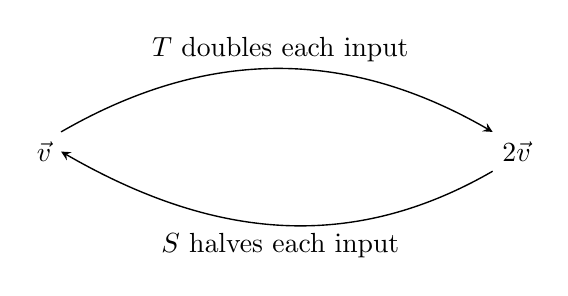
\begin{tikzpicture}
 \node[] at (0, -1.2)  (top)    {$T$ doubles each input};
 \node[] at (-3, -2.5)  (left1)    {$\vec{v}$};
 \node[] at (3, -2.5)  (right1)    {$2\vec{v}$};
 \node[] at (0, -3.7)  (bottom)    {$S$ halves each input};
  \draw [->,line width=0.5pt,-stealth]  (left1.north east)to[out=30, in=150](right1.north west);
 \draw [->,line width=0.5pt,-stealth]  (right1.south west)to[out=210, in=330](left1.east);
 \end{tikzpicture}
 \end{center} 

This gives us a way of thinking about an inverse of $T$ as a transformation that ``undoes" the action of $T$ by ``reversing" the mapping arrows.  We will now use these intuitive ideas to understand which linear transformations are invertible and which are not.

Given an arbitrary linear transformation $T:V\rightarrow W$, ``reversing the arrows"
 may not always result in a transformation. Recall that transformations are functions.  The figures below show two ways in which our attempt to ``reverse" $T$ may fail to produce a function.
 
 First, if two distinct vectors $\vec{v}_1$ and $\vec{v}_2$ map to the same vector $\vec{w}$ in $W$, then reversing the arrows gives us a mapping that is clearly not a function. 
 

\begin{center}
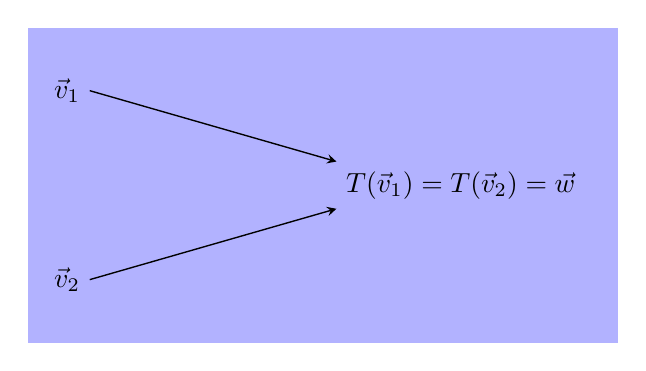
\begin{tikzpicture}
\fill[blue, opacity=0.3] (-5.5,-2) rectangle (2,2);
 \node[] at (-5, 1.2)  (topleft)    {$\vec{v}_1$};
 \node[] at (-5, -1.2)  (bottomleft)    {$\vec{v}_2$};
 \node[] at (0, 0)  (cleft1)    {$T(\vec{v}_1)=T(\vec{v}_2)=\vec{w}$};
 
% \node[gray] at (-5, 0)  (comment)    {(Two distinct elements map to $\vec{w}$)};
   \draw [->,line width=0.5pt,-stealth]  (topleft.east) to (cleft1.north west);
  \draw [->,line width=0.5pt,-stealth]  (bottomleft.east) to (cleft1.south west);
 \end{tikzpicture}
 \end{center} 
 
 \begin{center}
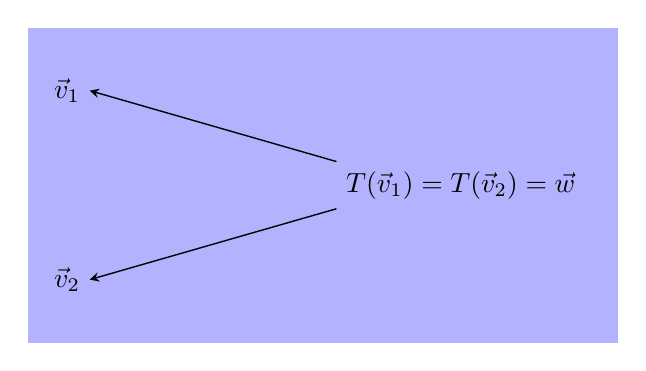
\begin{tikzpicture}
\fill[blue, opacity=0.3] (-5.5,-2) rectangle (2,2);
 \node[] at (-5, 1.2)  (topleft)    {$\vec{v}_1$};
 \node[] at (-5, -1.2)  (bottomleft)    {$\vec{v}_2$};
 \node[] at (0, 0)  (cleft1)    {$T(\vec{v}_1)=T(\vec{v}_2)=\vec{w}$};
% \node[gray] at (-6, 0)  (comment)    {(Reversing the arrows does not produce a function)};
   \draw [->,line width=0.5pt,-stealth]  (cleft1.north west) to (topleft.east);
  \draw [->,line width=0.5pt,-stealth]  (cleft1.south west) to (bottomleft.east);
  % \node[] at (-4, -2.5)  (caption)    {Figure 1.  When two distinct elements map to $\vec{w}$,};
  % \node[] at (-4, -3)  (caption) {reversing the arrows does not produce a function.};
 \end{tikzpicture}
 \end{center} 

  Based on this diagram, it is reasonable to conjecture that for a transformation to be invertible, the transformation must be such that each output is the image of exactly one input.  Such transformations are called \dfn{one-to-one}. 

\begin{definition}[One-to-One]\label{def:onetoone} A linear transformation $T:V\rightarrow W$ is \dfn{one-to-one} if 
$$T(\vec{v}_1)=T(\vec{v}_2)\quad \text{implies that}\quad \vec{v}_1=\vec{v}_2$$
\end{definition}  

Second, observe that our definition of an inverse of $T:V\rightarrow W$ requires that the domain of the inverse transformation be $W$. (Definition \ref{def:inverse}, \href{https://ximera.osu.edu/linearalgebradzv3/LinearAlgebraInteractiveIntro/LTR-0030/main}{Composition and Inverses of Linear Transformations})  If there is a vector $\vec{b}$ in $W$ that is not an image of any vector in $V$, then $\vec{b}$ cannot be in the domain of an inverse transformation. 

\begin{center}
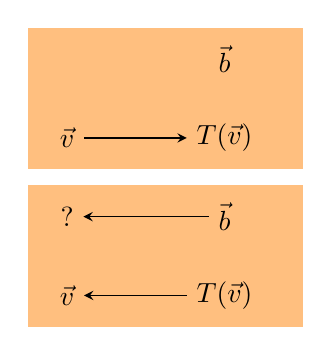
\begin{tikzpicture}
\fill[orange, opacity=0.5] (-2.5,1.6) rectangle (1,3.4);
 \node[] at (0, 3)  (topleft)    {$\vec{b}$};
 \node[] at (-2, 2)  (bottomleft)    {$\vec{v}$};
 \node[] at (0, 2)  (cleft1)    {$T(\vec{v})$};
%  \node[gray] at (2, 3)  (comment)    {(Nothing maps to $\vec{b}$)};
\fill[orange, opacity=0.5] (-2.5,-0.4) rectangle (1,1.4);
  \draw [->,line width=0.5pt,-stealth]  (bottomleft.east) to (cleft1.west);
  \node[] at (0, 1)  (topright)    {$\vec{b}$};
 \node[] at (-2, 0)  (bottomleft)    {$\vec{v}$};
 \node[] at (-2, 1)  (topleft)    {?};
 \node[] at (0, 0)  (cleft1)    {$T(\vec{v})$};
% \node[gray] at (3, 1)  (comment)    {($\vec{b}$ has nothing to map ``back" to)};
  
  \draw [->,line width=0.5pt,-stealth]  (cleft1.west) to (bottomleft.east);
  \draw [->,line width=0.5pt,-stealth]  (topright.west) to (topleft.east);
%  \node[] at (0, -1)  (caption)    {Figure 2.  What happens when nothing maps to $\vec{b}$.};
 \end{tikzpicture}
 \end{center}

The above figure makes a convincing case that for a transformation to be invertible every element of the codomain must have something mapping to it. Transformations such that every element of the codomain is an image of some element of the domain are called \dfn{onto}.

\begin{definition}[Onto]\label{def:onto} A linear transformation $T:V\rightarrow W$ is \dfn{onto} if for every element $\vec{w}$ of $W$, there exists an element $\vec{v}$ of $V$ such that $T(\vec{v})=\vec{w}$.
\end{definition}

\begin{theorem}\label{th:isomeansinvert} Let $V$ and $W$ be vector spaces, and let $T:V\rightarrow W$ be a linear transformation.  Then $T$ has an inverse if and only if $T$ is one-to-one and onto. 
\end{theorem}
\begin{proof}
We will first assume that $T$ is one-to-one and onto, and show that there exists a transformation $S:W\rightarrow V$ such that $S\circ T=\id_V$ and $T\circ S=\id_W$.  Because $T$ is onto, for every $\vec{w}$ in $W$, there exists $\vec{v}$ in $V$ such that $T(\vec{v})=\vec{w}$.  Moreover, because $T$ is one-to-one, vector $\vec{v}$ is the only vector that maps to $\vec{w}$.  To stress this, we will say that for every $\vec{w}$, there exists $\vec{v}_{\vec{w}}$ such that $T(\vec{v}_{\vec{w}})=\vec{w}$. (Since every $\vec{v}$ maps to exactly one $\vec{w}$, this notation makes sense for elements of $V$ as well.)  We can now define $S:W\rightarrow V$ by $S(\vec{w})=\vec{v}_{\vec{w}}$.
Then
$$(S\circ T)(\vec{v}_{\vec{w}})=S(T(\vec{v}_{\vec{w}}))=S(\vec{w})=\vec{v}_{\vec{w}}$$
$$(T\circ S)(\vec{w})=T(S(\vec{w}))=T(\vec{v}_{\vec{w}})=\vec{w}$$
We conclude that $S\circ T=\id_V$ and $T\circ S=\id_W$.  Therefore $S$ is an inverse of $T$.

We will now assume that $T$ has an inverse $S$ and show that $T$ must be one-to-one and onto.  
Suppose $$T(\vec{v}_1)=T(\vec{v}_2)$$ then $$S(T(\vec{v}_1))=S(T(\vec{v}_2))$$
but then
$$\vec{v}_1=\vec{v}_2$$
We conclude that $T$ is one-to-one.

Now suppose that $\vec{w}$ is in $W$.  We need to show that some element of $V$ maps to $\vec{w}$.  Let $\vec{v}=S(\vec{w})$.  Then
$$T(\vec{v})=T(S(\vec{w}))=(T\circ S)(\vec{w})=\id_W(\vec{w})=\vec{w}$$
We conclude that $T$ is onto.
\end{proof}

\begin{theorem}\label{ex:coordmapiso}
Let $V$ be a vector space, and let $\mathcal{B}$ be an ordered basis for $V$.  Then  the linear transformation $T:V\rightarrow \RR^n$ given by $T(\vec{v})=[\vec{v}]_{\mathcal{B}}$ is invertible.
\end{theorem}
\begin{proof}
We leave the proof of this result to the reader. 
\end{proof}
%%%%%%%%%%%%%%%%%%%%%%%



\begin{example}\label{example:isomorph}
Recall that the set of all polynomials of degree $2$ or less, together with polynomial addition and scalar multiplication, is a vector space, denoted by $\mathbb{P}^2$.  Let $\mathcal{B}=\{1, x, x^2\}$. You should do a quick mental check that $\mathcal{B}$ is a basis of $\mathbb{P}^2$.

Define a transformation $T:\mathbb{P}^2\rightarrow \RR^3$ by
$T(a+bx+cx^2)=\begin{bmatrix}a\\b\\c\end{bmatrix}$.  In other words, $T$ maps each element of $\mathbb{P}^2$ to its coordinate vector with respect to the ordered basis $\mathcal{B}$.  

The diagram below illustrates the actions of $T$ and $T^{-1}$ on several elements.
  
 \begin{center}
 \begin{tikzpicture} 
   \fill[blue, opacity=0.3] (0,0) rectangle (5,5);
   \fill[orange, opacity=0.5] (6,0) rectangle (11,5);
   
   \node[] at (0.5, 4.5)  (p2)    {$\mathbb{P}^2$};
   \node[] at (10.5, 4.5)  (r3)    {$\RR^3$};
   
   \node[] at (2.5, 4.2)  (p_1)    {$1+2x-3x^2$};
   \node[] at (1.2, 2.8)  (p_2)    {$-4$};
    \node[] at (3, 1.8)  (p_3)    {$x+5$};
     \node[] at (2, 0.6)  (p_4)    {$a+bx+cx^2$};
     
     \node[] at (8.5, 4.2)  (v_1)    {$\begin{bmatrix}1\\2\\-3\end{bmatrix}$};
   \node[] at (7.2, 3.2)  (v_2)    {$\begin{bmatrix}-4\\0\\0\end{bmatrix}$};
    \node[] at (9, 1.9)  (v_3)    {$\begin{bmatrix}5\\1\\0\end{bmatrix}$};
     \node[] at (7.5, 0.8)  (v_4)    {$\begin{bmatrix}a\\b\\c\end{bmatrix}$};
     
     \draw [->,line width=0.5pt,-stealth]  (3.6, 4.2)to[out=10, in=170](7.9,4.2);
     \draw [->,line width=0.5pt,-stealth]  (p_2.east)to[out=10, in=170](v_2.west);
     \draw [->,line width=0.5pt,-stealth]  (p_3.east)to[out=10, in=170](v_3.west);
     \draw [->,line width=0.5pt,-stealth]  (p_4.east)to[out=10, in=170](v_4.west);
     
     \draw [->,line width=0.5pt,-stealth]  (7.9,4.1)to[out=190, in=350](3.6, 4.1);
     \draw [->,line width=0.5pt,-stealth]  (6.5,3.1)to[out=190, in=350](1.6,2.7 );
     \draw [->,line width=0.5pt,-stealth]  (8.5,1.8)to[out=190, in=350](3.6,1.7 );
     \draw [->,line width=0.5pt,-stealth]  (7,0.7)to[out=190, in=350](3,0.5 );
     
     \draw [->,line width=0.5pt,-stealth]  (8.5,-0.1)to[out=200, in=340](2.5,-0.1 );
     \draw [->,line width=0.5pt,-stealth]  (2.5,5.1)to[out=20, in=160](8.5, 5.1);
     
     \node[] at (5.5, 6)    {$T$};
      \node[] at (5.5, -1)    {$T^{-1}$};
  \end{tikzpicture}
\end{center}

\end{example}

\subsection*{Coordinate Isomorphisms}

Invertible linear transformations, such as the coordinate mapping, are useful because they preserve the structure of interactions between elements as we move back and forth between two vector spaces, allowing us to answer questions about one vector space in a different vector space.  In particular, any question related to linear combinations can be addressed in this fashion. This includes questions concerning linear independence, span, basis and dimension. Specifically, for coordinate mappings, it is easy to see that the following property holds.

\begin{theorem}\label{th:coordmappingisoprop}
    Let $V$ be an $n$-dimensional vector space, and let $T:V\rightarrow \RR^n$ be the coordinate mapping with respect to some ordered basis $\mathcal{B}$ of $V$.  Then
    the set of vectors $\{\vec{x}_1,\vec{x}_2,\dots ,\vec{x}_k\}$ of $V$ is linearly independent if and only if the set $\{T(\vec{x}_1),T(\vec{x}_2),\dots ,T(\vec{x}_k)\}$ is linearly independent in $\RR^n$.
\end{theorem}

\begin{definition}\label{def:isomorphism} Let $V$ and $W$ be vector spaces.  If there exists an invertible linear transformation $T:V\rightarrow W$ we say that $V$ and $W$ are \dfn{isomorphic} and write $V\cong W$.  The invertible linear transformation $T$ is called an \dfn{isomorphism}.
\end{definition}

It is worth pointing out that if $T:V\rightarrow W$ is an isomorphism, then $T^{-1}:W\rightarrow V$, being linear and invertible, is also an isomorphism.

Because coordinate mappings are isomorphisms, we have the following fundamental result.

\begin{theorem}\label{th:ndimisotorn}
Every $n$-dimensional vector space is isomorphic to $\RR^n$.
\end{theorem}



\section*{Practice Problems}

\begin{problem}\label{prob:symmMatLinTrans}
Recall that the set $V$ of all symmetric $2\times 2$ matrices is a subspace of $\mathbb{M}_{2,2}$.  In Example \ref{ex:symmetricmatsubspace} of \href{https://ximera.osu.edu/linearalgebradzv3/LinearAlgebraInteractiveIntro/VSP-0060/main}{Bases and Dimension of Abstract Vector Spaces} we demonstrated that $\mathcal{B} = \left\{
\begin{bmatrix}
1 & 0 \\
0 & 0
\end{bmatrix}, \begin{bmatrix}
0 & 0 \\
0 & 1
\end{bmatrix}, \begin{bmatrix}
0 & 1 \\
1 & 0
\end{bmatrix}
\right\}$ is a basis for $V$.  Define $T:V\rightarrow \RR^3$ by $T(A)=[A]_{\mathcal{B}}$.  Find $T(I_2)$ and $T\left(\begin{bmatrix}2&-3\\-3&1\end{bmatrix}\right)$.

Answer:
$$T(I_2)=\begin{bmatrix}\answer{1}\\\answer{1}\\\answer{0}\end{bmatrix}$$
$$T\left(\begin{bmatrix}2&-3\\-3&1\end{bmatrix}\right)=\begin{bmatrix}\answer{2}\\\answer{1}\\\answer{-3}\end{bmatrix}$$
\end{problem}

\begin{problem}\label{prob:coordvector}
Let $V$ be a subspace of $\RR^3$ with a basis $\mathcal{B}=\left\{\begin{bmatrix}2\\1\\-1\end{bmatrix}, \begin{bmatrix}0\\3\\2\end{bmatrix}\right\}$.  Find the coordinate vector, $[\vec{v}]_{\mathcal{B}}$, for $\vec{v}=\begin{bmatrix}4\\-1\\-4\end{bmatrix}$.
$$[\vec{v}]_{\mathcal{B}}=\begin{bmatrix}\answer{2}\\\answer{-1}\end{bmatrix}$$

If the order of the basis elements in $\mathcal{B}$ were switched to form a new basis
$$\mathcal{B}'=\left\{\begin{bmatrix}0\\3\\2\end{bmatrix}, \begin{bmatrix}2\\1\\-1\end{bmatrix} \right\}$$
How would this affect the coordinate vector for $\vec{v}$?

$$[\vec{v}]_{\mathcal{B}'}=\begin{bmatrix}\answer{-1}\\\answer{2}\end{bmatrix}$$
\end{problem}



\begin{problem}\label{prob:polylintranscoordvect} Verify that
$\mathcal{B}=\{x^{2}, x + 1, 1 - x - x^{2}\}$ is a basis for $\mathbb{P}^2$.  Define $T:\mathbb{P}^2\rightarrow \RR^3$ by $T(p(x))=[p(x)]_{\mathcal{B}}$.  Find $T(0)$, $T(x+1)$ and $T(x^2-3x+1)$.

Answer:
$$T(0)=\begin{bmatrix}\answer{0}\\\answer{0}\\\answer{0}\end{bmatrix}$$
$$T(x+1)=\begin{bmatrix}\answer{0}\\\answer{1}\\\answer{0}\end{bmatrix}$$
$$T(x^2-3x+1)=\begin{bmatrix}\answer{3}\\\answer{-1}\\\answer{2}\end{bmatrix}$$
\end{problem}

\begin{problem}\label{prob:lintransandbasis4} Let $V$ and $W$ be vector spaces, and let $\mathcal{B}_V=\{\vec{v}_1, \vec{v}_2, \vec{v}_3, \vec{v}_4\}$ and $\mathcal{B}_W=\{\vec{w}_1,\vec{w}_2, \vec{w}_3\}$ be ordered bases of $V$ and $W$, respectively.  Suppose $T:V\rightarrow W$ is a linear transformation such that: $$T(\vec{v}_1)=\vec{w}_2$$ $$T(\vec{v}_2)=2\vec{w}_1-3\vec{w}_2$$
$$T(\vec{v}_3)=\vec{w}_2+\vec{w}_3$$
$$T(\vec{v}_4)=-\vec{w}_1$$
If $\vec{v}=-2\vec{v}_1+3\vec{v}_2-\vec{v}_4$, express $T(\vec{v})$ as a linear combination of vectors of $\mathcal{B}_W$.
$$T(\vec{v})=\answer{7}\vec{w}_1-\answer{11}\vec{w}_2+\answer{0}\vec{w}_3$$
Find $[\vec{v}]_{\mathcal{B}_V}$ and $[T(\vec{v})]_{\mathcal{B}_{W}}$
$$[\vec{v}]_{\mathcal{B}_V}=\begin{bmatrix}\answer{-2}\\\answer{3}\\\answer{0}\\\answer{-1}\end{bmatrix},\quad [T(\vec{v})]_{\mathcal{B}_{W}}=\begin{bmatrix}\answer{7}\\\answer{-11}\\\answer{0}\end{bmatrix}$$
\end{problem}

\begin{problem}\label{prob:useisoshowlinind}
Let 
$$\mathcal{S}=\left\{\begin{bmatrix}1&-3\\-2&2\end{bmatrix}, \begin{bmatrix}4&-2\\1&5\end{bmatrix}, \begin{bmatrix}5&5\\8&4\end{bmatrix}\right\}$$
Is $\mathcal{S}$ linearly independent in $\mathbb{M}_{2,2}$?  \wordChoice{\choice[correct]{Yes}\choice{No}}
\end{problem}

\begin{problem}\label{prob:basism22iso}
Let 
$$\mathcal{S}=\left\{\begin{bmatrix}1&2\\3&4\end{bmatrix}, \begin{bmatrix}5&6\\7&8\end{bmatrix}, \begin{bmatrix}9&10\\11&12\end{bmatrix}, \begin{bmatrix}13&14\\15&16\end{bmatrix}\right\}$$
Is $\mathcal{S}$ a basis for $\mathbb{M}_{2,2}$? \wordChoice{\choice{Yes}\choice[correct]{No}}
\end{problem}

\end{document}
